\documentclass[twoside]{book}

% Packages required by doxygen
\usepackage{fixltx2e}
\usepackage{calc}
\usepackage{doxygen}
\usepackage[export]{adjustbox} % also loads graphicx
\usepackage{graphicx}
\usepackage[utf8]{inputenc}
\usepackage{makeidx}
\usepackage{multicol}
\usepackage{multirow}
\PassOptionsToPackage{warn}{textcomp}
\usepackage{textcomp}
\usepackage[nointegrals]{wasysym}
\usepackage[table]{xcolor}

% NLS support packages
\usepackage[french]{babel}

% Font selection
\usepackage[T1]{fontenc}
\usepackage[scaled=.90]{helvet}
\usepackage{courier}
\usepackage{amssymb}
\usepackage{sectsty}
\renewcommand{\familydefault}{\sfdefault}
\allsectionsfont{%
  \fontseries{bc}\selectfont%
  \color{darkgray}%
}
\renewcommand{\DoxyLabelFont}{%
  \fontseries{bc}\selectfont%
  \color{darkgray}%
}
\newcommand{\+}{\discretionary{\mbox{\scriptsize$\hookleftarrow$}}{}{}}

% Page & text layout
\usepackage{geometry}
\geometry{%
  a4paper,%
  top=2.5cm,%
  bottom=2.5cm,%
  left=2.5cm,%
  right=2.5cm%
}
\tolerance=750
\hfuzz=15pt
\hbadness=750
\setlength{\emergencystretch}{15pt}
\setlength{\parindent}{0cm}
\setlength{\parskip}{3ex plus 2ex minus 2ex}
\makeatletter
\renewcommand{\paragraph}{%
  \@startsection{paragraph}{4}{0ex}{-1.0ex}{1.0ex}{%
    \normalfont\normalsize\bfseries\SS@parafont%
  }%
}
\renewcommand{\subparagraph}{%
  \@startsection{subparagraph}{5}{0ex}{-1.0ex}{1.0ex}{%
    \normalfont\normalsize\bfseries\SS@subparafont%
  }%
}
\makeatother

% Headers & footers
\usepackage{fancyhdr}
\pagestyle{fancyplain}
\fancyhead[LE]{\fancyplain{}{\bfseries\thepage}}
\fancyhead[CE]{\fancyplain{}{}}
\fancyhead[RE]{\fancyplain{}{\bfseries\leftmark}}
\fancyhead[LO]{\fancyplain{}{\bfseries\rightmark}}
\fancyhead[CO]{\fancyplain{}{}}
\fancyhead[RO]{\fancyplain{}{\bfseries\thepage}}
\fancyfoot[LE]{\fancyplain{}{}}
\fancyfoot[CE]{\fancyplain{}{}}
\fancyfoot[RE]{\fancyplain{}{\bfseries\scriptsize Généré par Doxygen }}
\fancyfoot[LO]{\fancyplain{}{\bfseries\scriptsize Généré par Doxygen }}
\fancyfoot[CO]{\fancyplain{}{}}
\fancyfoot[RO]{\fancyplain{}{}}
\renewcommand{\footrulewidth}{0.4pt}
\renewcommand{\chaptermark}[1]{%
  \markboth{#1}{}%
}
\renewcommand{\sectionmark}[1]{%
  \markright{\thesection\ #1}%
}

% Indices & bibliography
\usepackage{natbib}
\usepackage[titles]{tocloft}
\setcounter{tocdepth}{3}
\setcounter{secnumdepth}{5}
\makeindex

% Hyperlinks (required, but should be loaded last)
\usepackage{ifpdf}
\ifpdf
  \usepackage[pdftex,pagebackref=true]{hyperref}
\else
  \usepackage[ps2pdf,pagebackref=true]{hyperref}
\fi
\hypersetup{%
  colorlinks=true,%
  linkcolor=blue,%
  citecolor=blue,%
  unicode%
}

% Custom commands
\newcommand{\clearemptydoublepage}{%
  \newpage{\pagestyle{empty}\cleardoublepage}%
}

\usepackage{caption}
\captionsetup{labelsep=space,justification=centering,font={bf},singlelinecheck=off,skip=4pt,position=top}

%===== C O N T E N T S =====

\begin{document}

% Titlepage & ToC
\hypersetup{pageanchor=false,
             bookmarksnumbered=true,
             pdfencoding=unicode
            }
\pagenumbering{roman}
\begin{titlepage}
\vspace*{7cm}
\begin{center}%
{\Large Enigme\+\_\+2 \\[1ex]\large 1 }\\
\vspace*{1cm}
{\large Généré par Doxygen 1.8.11}\\
\end{center}
\end{titlepage}
\clearemptydoublepage
\tableofcontents
\clearemptydoublepage
\pagenumbering{arabic}
\hypersetup{pageanchor=true}

%--- Begin generated contents ---
\chapter{Index des fichiers}
\section{Liste des fichiers}
Liste de tous les fichiers avec une brève description \+:\begin{DoxyCompactList}
\item\contentsline{section}{\hyperlink{enigme__clavier_8c}{enigme\+\_\+clavier.\+c} \\*Writing Program }{\pageref{enigme__clavier_8c}}{}
\item\contentsline{section}{\hyperlink{enigme__clavier_8h}{enigme\+\_\+clavier.\+h} }{\pageref{enigme__clavier_8h}}{}
\item\contentsline{section}{\hyperlink{main_8c}{main.\+c} \\*Testing Program }{\pageref{main_8c}}{}
\end{DoxyCompactList}

\chapter{Documentation des fichiers}
\hypertarget{enigme__clavier_8c}{}\section{Référence du fichier enigme\+\_\+clavier.\+c}
\label{enigme__clavier_8c}\index{enigme\+\_\+clavier.\+c@{enigme\+\_\+clavier.\+c}}


Writing Program.  


{\ttfamily \#include $<$stdio.\+h$>$}\\*
{\ttfamily \#include $<$stdlib.\+h$>$}\\*
{\ttfamily \#include $<$S\+D\+L/\+S\+D\+L.\+h$>$}\\*
{\ttfamily \#include $<$S\+D\+L/\+S\+D\+L\+\_\+image.\+h$>$}\\*
{\ttfamily \#include $<$ctype.\+h$>$}\\*
{\ttfamily \#include $<$time.\+h$>$}\\*
{\ttfamily \#include $<$string.\+h$>$}\\*
{\ttfamily \#include $<$S\+D\+L/\+S\+D\+L\+\_\+ttf.\+h$>$}\\*
{\ttfamily \#include \char`\"{}enigme\+\_\+clavier.\+h\char`\"{}}\\*
Graphe des dépendances par inclusion de enigme\+\_\+clavier.\+c\+:
\nopagebreak
\begin{figure}[H]
\begin{center}
\leavevmode
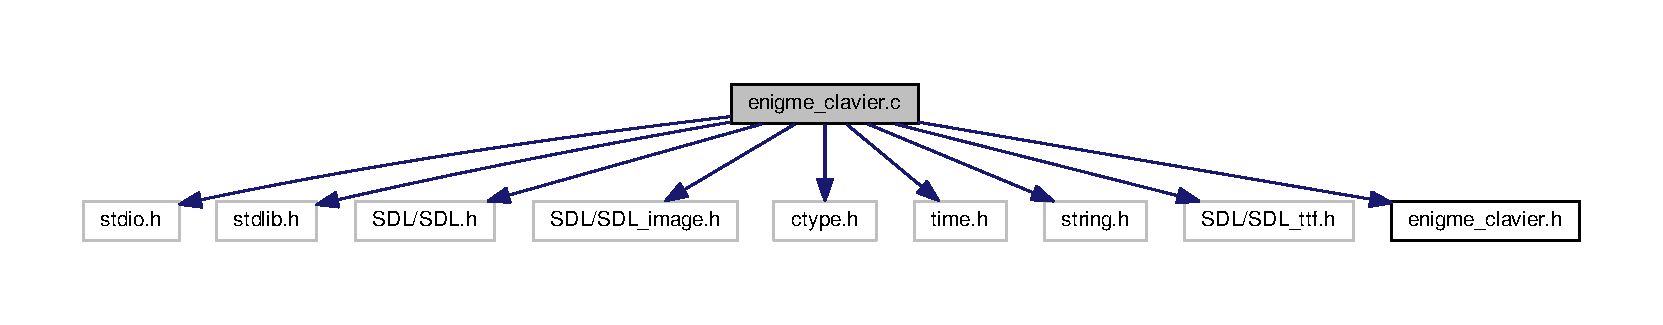
\includegraphics[width=350pt]{enigme__clavier_8c__incl}
\end{center}
\end{figure}
\subsection*{Fonctions}
\begin{DoxyCompactItemize}
\item 
int \hyperlink{enigme__clavier_8c_a6d388cc269cba866ddf559685d405be6}{afficher\+\_\+enigme} (S\+D\+L\+\_\+\+Surface $\ast$ecran, S\+D\+L\+\_\+\+Surface $\ast$chaine, T\+T\+F\+\_\+\+Font $\ast$police)
\begin{DoxyCompactList}\small\item\em Pour afficher enigme. \end{DoxyCompactList}\item 
int \hyperlink{enigme__clavier_8c_a36e5976175e9f189c2745ba884273dbe}{enigme\+\_\+clavier} (S\+D\+L\+\_\+\+Surface $\ast$ecran)
\begin{DoxyCompactList}\small\item\em Ecris le programme pour le resolution et affichage de l\textquotesingle{}enigme. \end{DoxyCompactList}\end{DoxyCompactItemize}


\subsection{Description détaillée}
Writing Program. 

\begin{DoxyAuthor}{Auteur}
Mintoua T Level-\/\+Up 
\end{DoxyAuthor}
\begin{DoxyVersion}{Version}
0.\+1 
\end{DoxyVersion}
\begin{DoxyDate}{Date}
Apr 21, 2019
\end{DoxyDate}
Writing program for enigme 

\subsection{Documentation des fonctions}
\index{enigme\+\_\+clavier.\+c@{enigme\+\_\+clavier.\+c}!afficher\+\_\+enigme@{afficher\+\_\+enigme}}
\index{afficher\+\_\+enigme@{afficher\+\_\+enigme}!enigme\+\_\+clavier.\+c@{enigme\+\_\+clavier.\+c}}
\subsubsection[{\texorpdfstring{afficher\+\_\+enigme(\+S\+D\+L\+\_\+\+Surface $\ast$ecran, S\+D\+L\+\_\+\+Surface $\ast$chaine, T\+T\+F\+\_\+\+Font $\ast$police)}{afficher_enigme(SDL_Surface *ecran, SDL_Surface *chaine, TTF_Font *police)}}]{\setlength{\rightskip}{0pt plus 5cm}int afficher\+\_\+enigme (
\begin{DoxyParamCaption}
\item[{S\+D\+L\+\_\+\+Surface $\ast$}]{ecran, }
\item[{S\+D\+L\+\_\+\+Surface $\ast$}]{chaine, }
\item[{T\+T\+F\+\_\+\+Font $\ast$}]{police}
\end{DoxyParamCaption}
)}\hypertarget{enigme__clavier_8c_a6d388cc269cba866ddf559685d405be6}{}\label{enigme__clavier_8c_a6d388cc269cba866ddf559685d405be6}


Pour afficher enigme. 

\begin{DoxyAuthor}{Auteur}
Mintoua T Level-\/\+Up 
\end{DoxyAuthor}

\begin{DoxyParams}{Paramètres}
{\em ecran} & .c\textquotesingle{}est l\textquotesingle{}écran du jeu \\
\hline
{\em chaine} & .Pour la question de l\textquotesingle{}enigme \\
\hline
{\em police} & .La police des textes \\
\hline
\end{DoxyParams}
\begin{DoxyDate}{Date}
Apr 21, 2019 
\end{DoxyDate}
\begin{DoxyReturn}{Renvoie}
numero de l\textquotesingle{}enigme(question) dans le fichier 
\end{DoxyReturn}


Voici le graphe des appelants de cette fonction \+:
\nopagebreak
\begin{figure}[H]
\begin{center}
\leavevmode
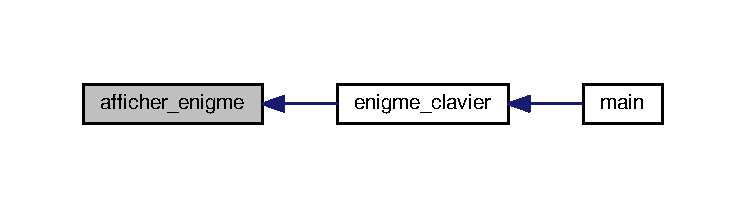
\includegraphics[width=350pt]{enigme__clavier_8c_a6d388cc269cba866ddf559685d405be6_icgraph}
\end{center}
\end{figure}


\index{enigme\+\_\+clavier.\+c@{enigme\+\_\+clavier.\+c}!enigme\+\_\+clavier@{enigme\+\_\+clavier}}
\index{enigme\+\_\+clavier@{enigme\+\_\+clavier}!enigme\+\_\+clavier.\+c@{enigme\+\_\+clavier.\+c}}
\subsubsection[{\texorpdfstring{enigme\+\_\+clavier(\+S\+D\+L\+\_\+\+Surface $\ast$ecran)}{enigme_clavier(SDL_Surface *ecran)}}]{\setlength{\rightskip}{0pt plus 5cm}int enigme\+\_\+clavier (
\begin{DoxyParamCaption}
\item[{S\+D\+L\+\_\+\+Surface $\ast$}]{ecran}
\end{DoxyParamCaption}
)}\hypertarget{enigme__clavier_8c_a36e5976175e9f189c2745ba884273dbe}{}\label{enigme__clavier_8c_a36e5976175e9f189c2745ba884273dbe}


Ecris le programme pour le resolution et affichage de l\textquotesingle{}enigme. 

\begin{DoxyAuthor}{Auteur}
Mintoua T Level-\/\+Up 
\end{DoxyAuthor}

\begin{DoxyParams}{Paramètres}
{\em ecran} & l\textquotesingle{}ecran du jeu \\
\hline
\end{DoxyParams}
\begin{DoxyReturn}{Renvoie}
entier (score ou vie) 
\end{DoxyReturn}
\begin{DoxyDate}{Date}
Apr 21, 2019
\end{DoxyDate}
Writing program for enigme 

Voici le graphe d\textquotesingle{}appel pour cette fonction \+:
\nopagebreak
\begin{figure}[H]
\begin{center}
\leavevmode
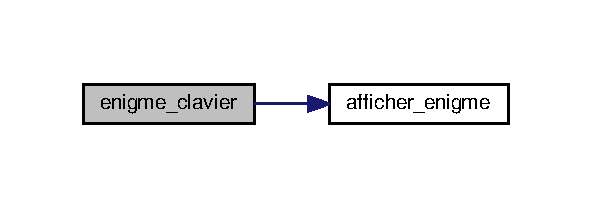
\includegraphics[width=284pt]{enigme__clavier_8c_a36e5976175e9f189c2745ba884273dbe_cgraph}
\end{center}
\end{figure}




Voici le graphe des appelants de cette fonction \+:
\nopagebreak
\begin{figure}[H]
\begin{center}
\leavevmode
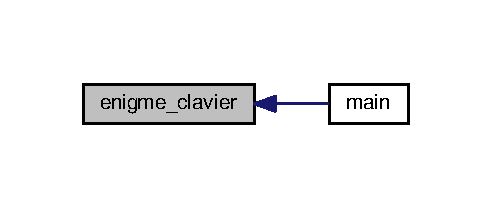
\includegraphics[width=236pt]{enigme__clavier_8c_a36e5976175e9f189c2745ba884273dbe_icgraph}
\end{center}
\end{figure}



\hypertarget{enigme__clavier_8h}{}\section{Référence du fichier enigme\+\_\+clavier.\+h}
\label{enigme__clavier_8h}\index{enigme\+\_\+clavier.\+h@{enigme\+\_\+clavier.\+h}}
Ce graphe montre quels fichiers incluent directement ou indirectement ce fichier \+:
\nopagebreak
\begin{figure}[H]
\begin{center}
\leavevmode
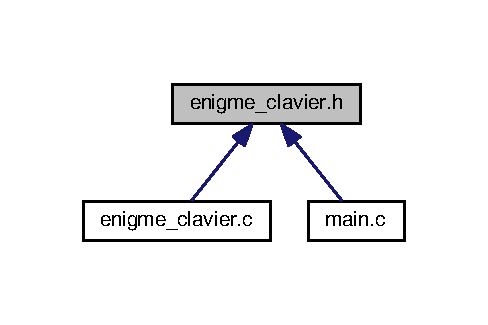
\includegraphics[width=234pt]{enigme__clavier_8h__dep__incl}
\end{center}
\end{figure}
\subsection*{Fonctions}
\begin{DoxyCompactItemize}
\item 
int \hyperlink{enigme__clavier_8h_a6d388cc269cba866ddf559685d405be6}{afficher\+\_\+enigme} (S\+D\+L\+\_\+\+Surface $\ast$ecran, S\+D\+L\+\_\+\+Surface $\ast$chaine, T\+T\+F\+\_\+\+Font $\ast$police)
\begin{DoxyCompactList}\small\item\em Pour afficher enigme. \end{DoxyCompactList}\item 
int \hyperlink{enigme__clavier_8h_ad9ebf69b0e14d7757c7480b1ee7cae09}{resolution} (int alea, S\+D\+L\+\_\+\+Surface $\ast$ecran, S\+D\+L\+\_\+\+Event event, S\+D\+L\+\_\+\+Surface $\ast$chaine, T\+T\+F\+\_\+\+Font $\ast$police)
\item 
int \hyperlink{enigme__clavier_8h_a36e5976175e9f189c2745ba884273dbe}{enigme\+\_\+clavier} (S\+D\+L\+\_\+\+Surface $\ast$ecran)
\begin{DoxyCompactList}\small\item\em Ecris le programme pour le resolution et affichage de l\textquotesingle{}enigme. \end{DoxyCompactList}\end{DoxyCompactItemize}


\subsection{Documentation des fonctions}
\index{enigme\+\_\+clavier.\+h@{enigme\+\_\+clavier.\+h}!afficher\+\_\+enigme@{afficher\+\_\+enigme}}
\index{afficher\+\_\+enigme@{afficher\+\_\+enigme}!enigme\+\_\+clavier.\+h@{enigme\+\_\+clavier.\+h}}
\subsubsection[{\texorpdfstring{afficher\+\_\+enigme(\+S\+D\+L\+\_\+\+Surface $\ast$ecran, S\+D\+L\+\_\+\+Surface $\ast$chaine, T\+T\+F\+\_\+\+Font $\ast$police)}{afficher_enigme(SDL_Surface *ecran, SDL_Surface *chaine, TTF_Font *police)}}]{\setlength{\rightskip}{0pt plus 5cm}int afficher\+\_\+enigme (
\begin{DoxyParamCaption}
\item[{S\+D\+L\+\_\+\+Surface $\ast$}]{ecran, }
\item[{S\+D\+L\+\_\+\+Surface $\ast$}]{chaine, }
\item[{T\+T\+F\+\_\+\+Font $\ast$}]{police}
\end{DoxyParamCaption}
)}\hypertarget{enigme__clavier_8h_a6d388cc269cba866ddf559685d405be6}{}\label{enigme__clavier_8h_a6d388cc269cba866ddf559685d405be6}


Pour afficher enigme. 

\begin{DoxyAuthor}{Auteur}
Mintoua T Level-\/\+Up 
\end{DoxyAuthor}

\begin{DoxyParams}{Paramètres}
{\em ecran} & .c\textquotesingle{}est l\textquotesingle{}écran du jeu \\
\hline
{\em chaine} & .Pour la question de l\textquotesingle{}enigme \\
\hline
{\em police} & .La police des textes \\
\hline
\end{DoxyParams}
\begin{DoxyDate}{Date}
Apr 21, 2019 
\end{DoxyDate}
\begin{DoxyReturn}{Renvoie}
numero de l\textquotesingle{}enigme(question) dans le fichier 
\end{DoxyReturn}


Voici le graphe des appelants de cette fonction \+:
\nopagebreak
\begin{figure}[H]
\begin{center}
\leavevmode
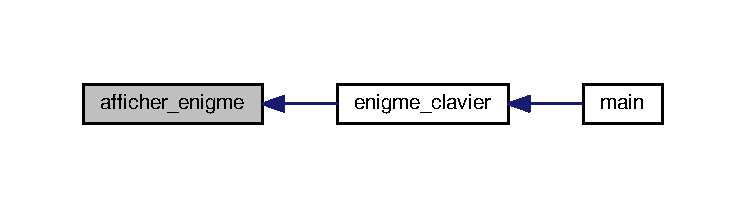
\includegraphics[width=350pt]{enigme__clavier_8h_a6d388cc269cba866ddf559685d405be6_icgraph}
\end{center}
\end{figure}


\index{enigme\+\_\+clavier.\+h@{enigme\+\_\+clavier.\+h}!enigme\+\_\+clavier@{enigme\+\_\+clavier}}
\index{enigme\+\_\+clavier@{enigme\+\_\+clavier}!enigme\+\_\+clavier.\+h@{enigme\+\_\+clavier.\+h}}
\subsubsection[{\texorpdfstring{enigme\+\_\+clavier(\+S\+D\+L\+\_\+\+Surface $\ast$ecran)}{enigme_clavier(SDL_Surface *ecran)}}]{\setlength{\rightskip}{0pt plus 5cm}int enigme\+\_\+clavier (
\begin{DoxyParamCaption}
\item[{S\+D\+L\+\_\+\+Surface $\ast$}]{ecran}
\end{DoxyParamCaption}
)}\hypertarget{enigme__clavier_8h_a36e5976175e9f189c2745ba884273dbe}{}\label{enigme__clavier_8h_a36e5976175e9f189c2745ba884273dbe}


Ecris le programme pour le resolution et affichage de l\textquotesingle{}enigme. 

\begin{DoxyAuthor}{Auteur}
Mintoua T Level-\/\+Up 
\end{DoxyAuthor}

\begin{DoxyParams}{Paramètres}
{\em ecran} & l\textquotesingle{}ecran du jeu \\
\hline
\end{DoxyParams}
\begin{DoxyReturn}{Renvoie}
entier (score ou vie) 
\end{DoxyReturn}
\begin{DoxyDate}{Date}
Apr 21, 2019
\end{DoxyDate}
Writing program for enigme 

Voici le graphe d\textquotesingle{}appel pour cette fonction \+:
\nopagebreak
\begin{figure}[H]
\begin{center}
\leavevmode
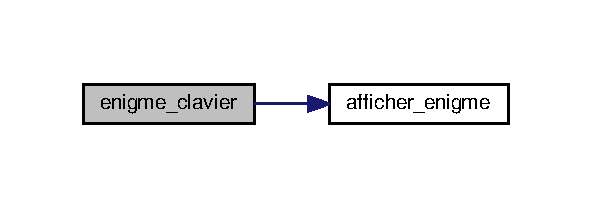
\includegraphics[width=284pt]{enigme__clavier_8h_a36e5976175e9f189c2745ba884273dbe_cgraph}
\end{center}
\end{figure}




Voici le graphe des appelants de cette fonction \+:
\nopagebreak
\begin{figure}[H]
\begin{center}
\leavevmode
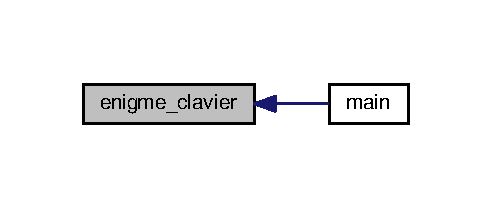
\includegraphics[width=236pt]{enigme__clavier_8h_a36e5976175e9f189c2745ba884273dbe_icgraph}
\end{center}
\end{figure}


\index{enigme\+\_\+clavier.\+h@{enigme\+\_\+clavier.\+h}!resolution@{resolution}}
\index{resolution@{resolution}!enigme\+\_\+clavier.\+h@{enigme\+\_\+clavier.\+h}}
\subsubsection[{\texorpdfstring{resolution(int alea, S\+D\+L\+\_\+\+Surface $\ast$ecran, S\+D\+L\+\_\+\+Event event, S\+D\+L\+\_\+\+Surface $\ast$chaine, T\+T\+F\+\_\+\+Font $\ast$police)}{resolution(int alea, SDL_Surface *ecran, SDL_Event event, SDL_Surface *chaine, TTF_Font *police)}}]{\setlength{\rightskip}{0pt plus 5cm}int resolution (
\begin{DoxyParamCaption}
\item[{int}]{alea, }
\item[{S\+D\+L\+\_\+\+Surface $\ast$}]{ecran, }
\item[{S\+D\+L\+\_\+\+Event}]{event, }
\item[{S\+D\+L\+\_\+\+Surface $\ast$}]{chaine, }
\item[{T\+T\+F\+\_\+\+Font $\ast$}]{police}
\end{DoxyParamCaption}
)}\hypertarget{enigme__clavier_8h_ad9ebf69b0e14d7757c7480b1ee7cae09}{}\label{enigme__clavier_8h_ad9ebf69b0e14d7757c7480b1ee7cae09}

\hypertarget{fichier__enigme_8txt}{}\section{Référence du fichier fichier\+\_\+enigme.\+txt}
\label{fichier__enigme_8txt}\index{fichier\+\_\+enigme.\+txt@{fichier\+\_\+enigme.\+txt}}

\hypertarget{main_8c}{}\section{Référence du fichier main.\+c}
\label{main_8c}\index{main.\+c@{main.\+c}}


Testing Program.  


{\ttfamily \#include $<$stdio.\+h$>$}\\*
{\ttfamily \#include $<$stdlib.\+h$>$}\\*
{\ttfamily \#include $<$S\+D\+L/\+S\+D\+L.\+h$>$}\\*
{\ttfamily \#include $<$S\+D\+L/\+S\+D\+L\+\_\+image.\+h$>$}\\*
{\ttfamily \#include $<$S\+D\+L/\+S\+D\+L\+\_\+ttf.\+h$>$}\\*
{\ttfamily \#include $<$string.\+h$>$}\\*
{\ttfamily \#include $<$ctype.\+h$>$}\\*
{\ttfamily \#include $<$time.\+h$>$}\\*
{\ttfamily \#include \char`\"{}enigme\+\_\+clavier.\+h\char`\"{}}\\*
Graphe des dépendances par inclusion de main.\+c\+:
\nopagebreak
\begin{figure}[H]
\begin{center}
\leavevmode
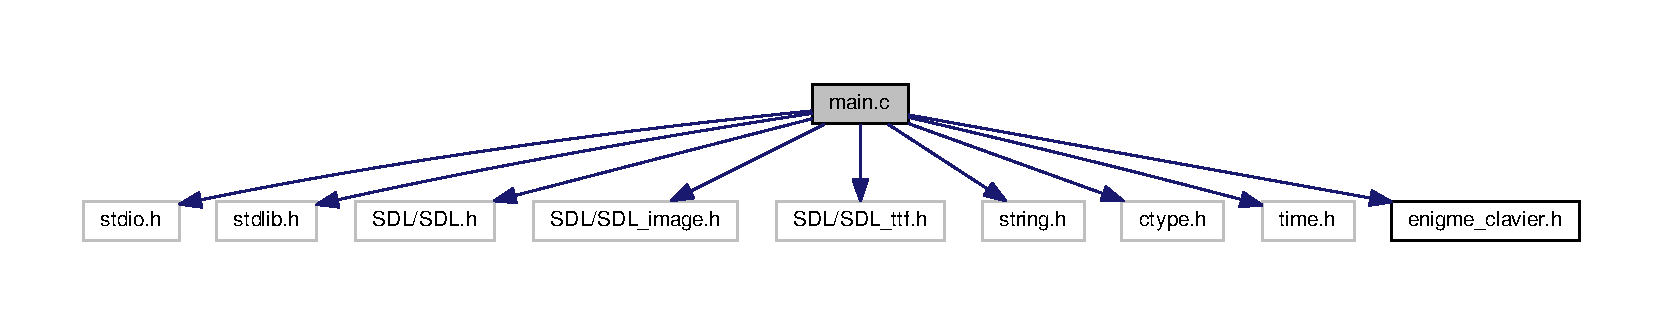
\includegraphics[width=350pt]{main_8c__incl}
\end{center}
\end{figure}
\subsection*{Fonctions}
\begin{DoxyCompactItemize}
\item 
int \hyperlink{main_8c_ae66f6b31b5ad750f1fe042a706a4e3d4}{main} ()
\end{DoxyCompactItemize}


\subsection{Description détaillée}
Testing Program. 

\begin{DoxyAuthor}{Auteur}
Mintoua T Level-\/\+Up 
\end{DoxyAuthor}
\begin{DoxyVersion}{Version}
0.\+1 
\end{DoxyVersion}
\begin{DoxyDate}{Date}
Apr 21, 2019
\end{DoxyDate}
Testing program for enigme 

\subsection{Documentation des fonctions}
\index{main.\+c@{main.\+c}!main@{main}}
\index{main@{main}!main.\+c@{main.\+c}}
\subsubsection[{\texorpdfstring{main()}{main()}}]{\setlength{\rightskip}{0pt plus 5cm}int main (
\begin{DoxyParamCaption}
{}
\end{DoxyParamCaption}
)}\hypertarget{main_8c_ae66f6b31b5ad750f1fe042a706a4e3d4}{}\label{main_8c_ae66f6b31b5ad750f1fe042a706a4e3d4}


Voici le graphe d\textquotesingle{}appel pour cette fonction \+:
\nopagebreak
\begin{figure}[H]
\begin{center}
\leavevmode
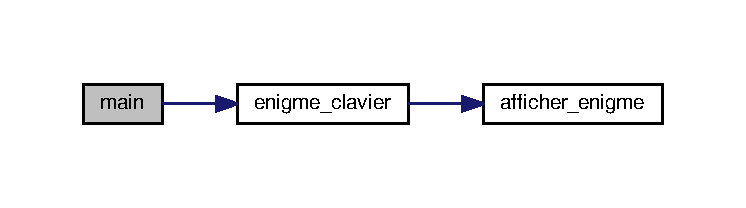
\includegraphics[width=350pt]{main_8c_ae66f6b31b5ad750f1fe042a706a4e3d4_cgraph}
\end{center}
\end{figure}



\hypertarget{reponse__enigme_8txt}{}\section{Référence du fichier reponse\+\_\+enigme.\+txt}
\label{reponse__enigme_8txt}\index{reponse\+\_\+enigme.\+txt@{reponse\+\_\+enigme.\+txt}}

%--- End generated contents ---

% Index
\backmatter
\newpage
\phantomsection
\clearemptydoublepage
\addcontentsline{toc}{chapter}{Index}
\printindex

\end{document}
